\documentclass{article}

\usepackage[margin=.75in]{geometry}
\usepackage{amsmath}
\usepackage{amssymb}
\usepackage[shortlabels]{enumitem}
\usepackage{pgfplots}
\usepackage{circuitikz}
\usepackage{float}
\usepackage{verbatim}

\author{Damien Prieur}
\title{Homework 8\\ ECES 512}
\date{}

\begin{document}

\maketitle

\section*{Problem 1}

\begin{tabular}{p{.45\textwidth}p{.45\textwidth}}
Consider the inverted pendulum as depicted in Fig. 1.
For small rotation angle $\theta$, the equation of motion is given by
\begin{gather*}
M\ell \ddot{\theta} = (M + m)g\theta -u \\
M \ddot{x} = u -mg\theta
\end{gather*}
Assume $M = 3\text{kg}$, $m = 0.75\text{kg}$, and $\ell = 1.5\text{m}$ and the state $x_1 = \theta,\quad x_2 = \dot{theta}, \quad x_3 = x, \quad x_4 = \dot{x}$, with output $y_1 = \theta$, and $y_2 = x$.
&
\raisebox{-.8\height}{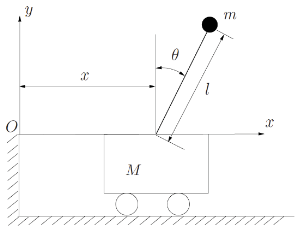
\includegraphics{images_static/inverted_pendulum_setup.png}}
\end{tabular}


\begin{enumerate}[a.]
\item Create a state space model for the system
\newline

\item Is the system stable?
Verify with plotting initial condition response in Matlab, with $x(0) = \begin{bmatrix} 0.05 \\ 0 \\ 0 \\ 0 \end{bmatrix}$.
If unstable, under what condition should we be able to stabilize the system.
How do we figure whether we can design an observer to the system?
\newline

\item Find the state feedback gain $K$ to put the closed-loop poles at $ -4 \pm 4j,\quad -25,\quad -25$.
Evaluate the performance of your controller by simulation via the initial condition response for $x(0) = \begin{bmatrix} 0.05 \\ 0 \\ 0 \\ 0 \end{bmatrix}$.
Also simulate and plot the step response of the controlled system.
\newline

\item Design and simulate a full order closed loop observer with $x(0) = \begin{bmatrix} 0.05 \\ 1 \\ -1 \\ 2 \end{bmatrix}$, but use $\begin{bmatrix} 0 \\ 0 \\ 0 \\ 0 \end{bmatrix}$ for the observer's initial states.
Put all the observer poles at $ (-50, -50, -100, -100)$.
Plot the state estimation error.
\newline

\item Design an output feedback controller using the observer designed in d.
Simulate and plot the step responses to different initial conditions for the state of te plant and the state of the observer.
Compare with c and discuss.
\newline

\end{enumerate}

\newpage

\section*{Problem 2}
Consider the mechanical system given in Figure 2, where $\xi_1, \xi_2$ are displacements of the masses, $u_1$ is the force acting on the masses.
Take the masses to be $m_1 = m_2 = 1\text{kg}$, the spring stiffness to be $k_1 = k_2 = 1 \frac{\text{N}}{\text{m}}$, and the damping coefficient to be $v = 1 \frac{\text{Ns}}{m}$.
\begin{figure}[h!]
\centering
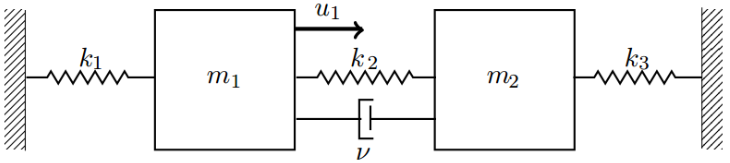
\includegraphics[width=.8\linewidth]{images_static/damped_mass_spring_system.png}
\end{figure}

$$ x(t) =
\begin{bmatrix}
\xi_1 \\
\xi_2 \\
\dot{\xi}_1 \\
\dot{\xi}_2 \\
\end{bmatrix}
\in \mathbb{R}^4
$$
$$ \ddot{\xi}_1 = -\xi_1 + (\xi_2 - \xi_1) + (\dot{\xi}_2 - \dot{\xi}_1) + u_1 $$
$$ \ddot{\xi}_2 = -\xi_2 + (\xi_1 - \xi_2) + (\dot{\xi}_1 - \dot{\xi}_2) $$

\begin{enumerate}[a.]
\item Create a state space model for the system. Consider both displacements as outputs $y_1,y_2$.
\newline

\item Is the system stable?
Verify with plotting initial condition response in Matlab, with $x(0) = \begin{bmatrix} 0.05 \\ 0 \\ 0.15 \\ 0 \end{bmatrix}$.
If unstable, under what condition should we be able to stabilize the system.
How do we figure whether we can design an observer to the system?
\newline

\item Find the state feedback gain $K$ to put the closed-loop poles at $ -4 \pm 4j,\quad -25,\quad -25$.
Evaluate the performance of your controller by simulation via the initial condition response for $x(0) = \begin{bmatrix} 0.05 \\ 0 \\ 0.15 \\ 0 \end{bmatrix}$.
Also simulate and plot the step response of the controlled system.
\newline

\item Design and simulate a full order closed loop observer with $x(0) = \begin{bmatrix} 0.05 \\ 0.01 \\ 0.15 \\ 0.01 \end{bmatrix}$, but use $\begin{bmatrix} 0 \\ 0 \\ 0 \\ 0 \end{bmatrix}$ for the observer's initial states.
Put all the observer poles at $ (-50, -50, -100, -100)$.
Plot the state estimation error.
\newline

\item Design an output feedback controller using the observer designed in d.
Simulate and plot the step responses to different initial conditions for the state of te plant and the state of the observer.
Compare with c and discuss.
\newline

\end{enumerate}

\end{document}
